\documentclass{beamer}

\usepackage[brazil]{babel}
\usepackage[utf8]{inputenc}
\usepackage{fancybox}
\usepackage{graphicx}
\usepackage{setspace}

\setstretch{1.25}
\graphicspath{ {./resources/} }


\newcommand{\fone}{\sum_{i=0}^{5} \left(100(x_{i+1} - x_{i}^{2})^2 + (1 - x_i)^2\right)}
\newcommand{\ftwo}{\sum_{i=0}^{99} x_i^4 - 16 x_i^2 + 5 x_i}
\newcommand{\fthree}{(x_0^2 + x_1 - 11)^2 + (x_0 + x_1^2 - 7)^2}
\newcommand{\R}{\mathbb{R}}

\usetheme{Pittsburgh}
\usecolortheme{owl}

\mode<presentation> { \setbeamercovered{transparent} }
\setbeamertemplate{navigation symbols}{}
\makeatletter
\beamer@centeredfalse
\def\beamerorig@set@color{%
  \pdfliteral{\current@color}%
  \aftergroup\reset@color
}
\def\beamerorig@reset@color{\pdfliteral{\current@color}}


\title[Otimização]
{Algoritmos de Otimização}

\subtitle{Aplicação de Algoritmos em funções específicas}

\author[Matheus Cardoso]
{M. Cardoso\inst{1}}

\institute[UFRJ]
{
  \inst{1}%
  Engenharia de Computação e Informação\\
  Universidade Federal do Rio de Janeiro
}

\date[2024]
{Novembro de 2024}

\begin{document}


\frame{\titlepage}


\begin{frame}[t]
\frametitle{As funções}

\begin{align*}
	\text{min} && f_1(x) &= \fone \\
	\text{s.a.} && x \in \R^7 \\
	\text{min} && f_2(x) &= \ftwo \\
	\text{s.a.} && x \in \R^{100} \\
	\text{min} && f_3(x) &= \fthree \\
	\text{s.a.} && x \in \R^2
\end{align*}

\end{frame}


\begin{frame}
\frametitle{Analisando a função $f_1$}
$f_1(x) = \fone$ \pause

Percebe-se que:
\[
	\left(100(x_{i+1} - x_{i}^{2})^2 + (1 - x_i)^2\right) \geq 0
\]

Pois $(10(x_{i+1} - x_{i}^{2}))^2 \geq 0$ e 
$(1 - x_i)^2 \geq 0$. \pause

($1 - x_i = 0$), logo $x_{i+1} = 1$ para zerar a primeira parcela.

O $x$ que garante o mínimo será $x^{T} = (1 \ 1 \ 1 \ 1 \ 1 \ 1 \ 1)$
\end{frame}


\begin{frame}
\frametitle{Analisando a função $f_1$}
Derivadas parciais e Hessiana.

\begin{align*}
	\frac{\partial f_1}{\partial x_0} = 400 x_0^3 - 400 x_0 x_1 + 2 x_0 - 2 \\
	\frac{\partial f_1}{\partial x_6} = -200 x_5^2 + 200 x_6 \\
	\frac{\partial f_1}{\partial x_i} = 400 x_i^3 - 400 x_i x_{i+1} - 200 x_{i-1}^2 + 202 x_i - 2, \\ \forall i \in \left\{1, 2, 3, 4, 5\right\}
\end{align*}

\end{frame}


\begin{frame}
\frametitle{Analisando a função $f_1$}
Derivadas parciais e Hessiana.
\begin{align*}
	\frac{\partial^2 f_1}{\partial x_i^2}                &= 1200 x_i^2 - 400 x_{i+1} + 202, \forall i \in \{1, 2, 3, 4, 5\}\\
	\frac{\partial^2 f_1}{\partial x_0^2}                &= 1200 x_0^2 - 400 x_{1} + 2 \\
	\frac{\partial^2 f_1}{\partial x_6^2}                &= 200 \\
	\frac{\partial^2 f_1}{\partial x_i \partial x_{i-1}} &= - 400 x_{i-1}, \forall i \in \left\{1, 2, 3, 4, 5, 6\right\}  \\
	\frac{\partial^2 f_1}{\partial x_i \partial x_{i+1}} &= - 400 x_i, \forall i \in \left\{0, 1, 2, 3, 4, 5\right\}
\end{align*}

\end{frame}

\begin{frame}
\frametitle{Analisando a função $f_2$}
\begin{align*}
	f_2(x) &= \ftwo
\end{align*} \pause

Como a função:
\[
	x_i^4 - 16 x_i^2 + 5 x_i
\]
já possui mínimo, o mínimo de $f_2$ será um vetor cujos valores
serão o $x$ que garante o mínimo para $x^4 - 16 x^2 + 5 x$ \pause

Plotemos
\end{frame}

\begin{frame}
\frametitle{Analisando a função $f_2$}

\begin{center}
	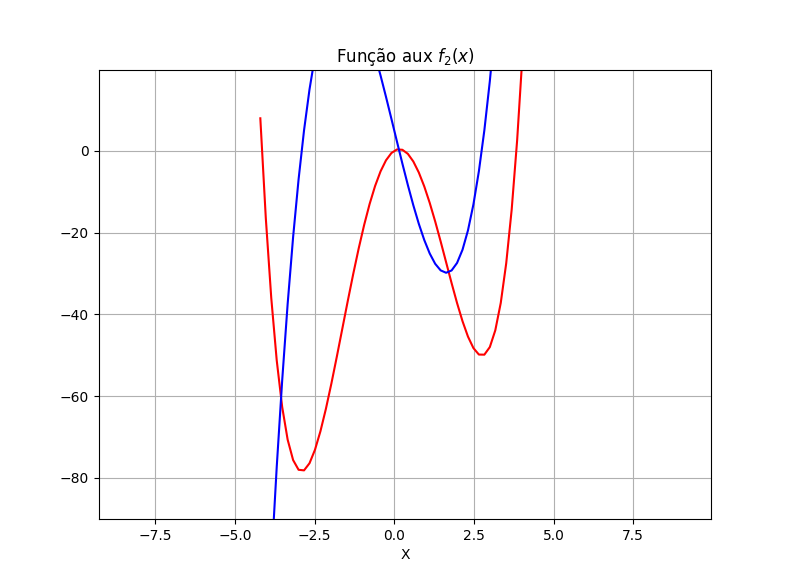
\includegraphics[scale=0.5]{fig1.png}
\end{center}
\end{frame}

\begin{frame}
\frametitle{Analisando a função $f_2$}

\begin{center}
	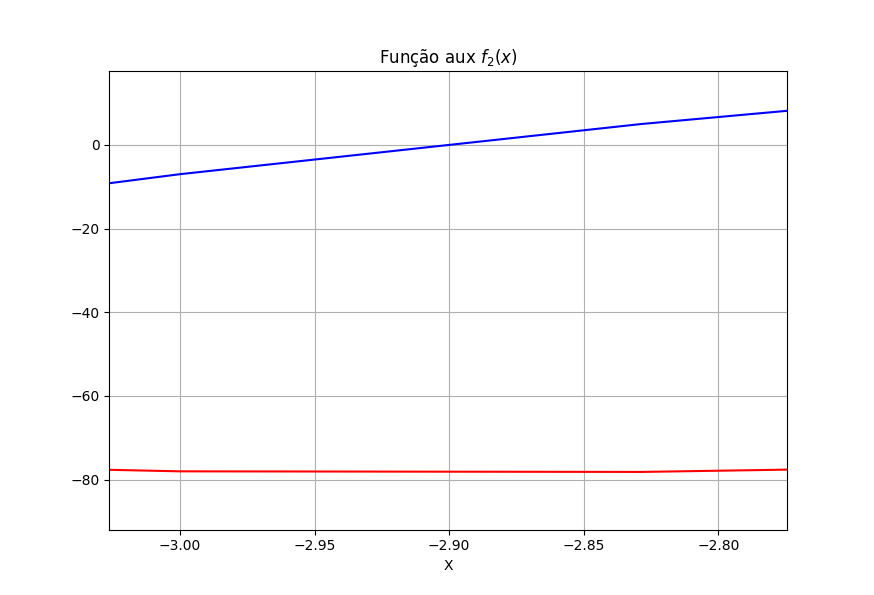
\includegraphics[scale=0.4]{fig2.png}
\end{center}

Para que a função seja mínima, $x \approx -2.9$ \pause

$x^T \approx (-2.9 \ -2.9 \ \cdots \ -2.9)$
\end{frame}

\begin{frame}
\frametitle{Analisando a função $f_2$}
Gradiente e Hessiana

\begin{align*}
	\frac{\partial f_2}{\partial x_i}     &= 4 x_i^3 - 32 x_i + 5, \forall i \in \left\{0, 1, \cdots, 99\right\} \\
	\vspace{0.5in} \\
	\frac{\partial^2 f_2}{\partial x_i^2} &= 12 x_i^2 - 32, \forall i \in \left\{0, 1, \cdots, 99\right\}
\end{align*}

\end{frame}

\begin{frame}
\frametitle{Analisando a função $f_3$}
$f_3(x) = \fthree$

Soma de dois quadrados, $f_3(x) \geq 0$ \pause
\begin{equation*}
\left\{
	\begin{aligned}
		& x_0^2 + x_1 - 11 = 0 \\
		& x_0 + x_1^2 - 7 = 0
	\end{aligned}	
\right.
\end{equation*} \pause
\begin{center}
	$(x_0 - 3)(x_0^3 + 3x_0^2 - 13x_0 -38) = 0 \ \ \ \ \ x_1 = 11 - x_0^2$
\end{center}
\begin{align*}
	x_a = \begin{pmatrix}
		3 \\
		2
	\end{pmatrix}
	&&
	x_b = \begin{pmatrix}
		-3.779 \\
		-3.280
	\end{pmatrix}
	&&
	x_c = \begin{pmatrix}
		-2.805 \\
		3.131
	\end{pmatrix}
	&&
	x_d = \begin{pmatrix}
		3.584 \\
		-1.845
	\end{pmatrix}
\end{align*}
\end{frame}


\begin{frame}
\frametitle{Analisando a função $f_3$}

Plotando a função $x^3 + 3x^2 - 13x - 38 = 0$

\begin{center}
	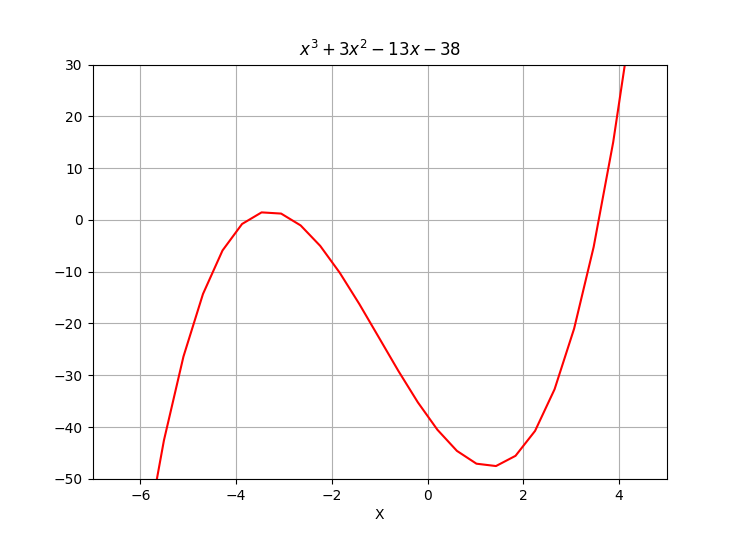
\includegraphics[scale=0.5]{fig3.png}
\end{center}

\end{frame}

\begin{frame}
\frametitle{Analisando a função $f_3$}

Gradiente e Hessiana

\begin{align*}
	\frac{\partial f_3}{\partial x_0} &= 4 x_0^3 + 4 x_0 x_1 - 42 x_0 + 2 x_1^2 - 14 \\
	\frac{\partial f_3}{\partial x_1} &= 4 x_1^3 + 4 x_0 x_1 - 26 x_1 + 2 x_0^2 - 22 \\
	\vspace{1in} \\
	\frac{\partial^2 f_3}{\partial x_0^2} &= 12 x_0^2 + 4 x_1 - 42 && \frac{\partial^2 f_3}{\partial x_0 \partial x_1} &= 4(x_0 + x_1) \\
	\frac{\partial^2 f_3}{\partial x_1^2} &= 12 x_1^2 + 4 x_0 - 26 && \frac{\partial^2 f_3}{\partial x_1 \partial x_0} &= 4(x_0 + x_1)
\end{align*}

\end{frame}

\begin{frame}
\frametitle{Testes - Gradiente}

\end{frame}

\end{document}
